\chapter{Fundamentals and Related Work}
\label{chap:fundamentals}
This chapter provides the fundamental concepts and related work that are required to understand the approach to be discussed in following Chapter \ref{chap:approach}. The first section introduces definitions of terms that are used throughout this document. The second section provides a brief introduction about the Informal Process Essentials (IPE) approach, as this provides basic information required for understanding this thesis work. The third section provides a short overview about organizational modeling notations mentioned in the another thesis work\cite{Sierr2015}. Though provided notations are not part of implementation, it is introduced to assist the reader in better understanding. The fourth section also describes about fundamental information required to understand the concepts of this thesis work. The fifth section discusses about the entity types representation of the organizational modeling. The last section discusses in details about each steps of the informal process modeling phase. 

%%%%%%%%%%%%%%%%%%%%%%%%%%%%%%%%%%%%%%%%%%%%%%%%%%%%%%%%%%%%%%%%%%%%%%%%%
\section{Definitions of Terms}
\label{sec:termdefinitions}
%%%%%%%%%%%%%%%%%%%%%%%%%%%%%%%%%%%%%%%%%%%%%%%%%%%%%%%%%%%%%%%%%%%%%%%%%
In this section, the definitions of terminologies that are used throughout this document are provided briefly.

\textit{Business Process} -  A business process has been defined as the set of activities whose final output is accomplishment of a goal \cite{Weske2012}.  

\textit{Business Logic} - Business logic refers to the activities that need to be done to execute the corresponding process. 

\textit{Business Process Models} - Business process models are models to capture recurring activities during a business process execution and enact them in a automated fashion for re-using those stored knowledge. 

\textit{Informal Process} - Informal processes are the processes whose execution steps cannot be modeled or are not feasible to model before their enactments. This is because due to the dynamic changing behavior during execution of the informal processes.  For example, software development process is an informal process, where required activities and order of their execution cannot be determined beforehand \cite{Sungur2015}.    

\textit{Informal Process Essentials} - Informal Process Essentials (IPE) is a resource-driven approach that enables describing process declaratively, i.e., without describing how the intention is achieved, and providing only information about what has to be achieved \cite{Sungur2014a}. 

\textit{OASIS Topology and Orchestration Specification for Cloud Applications} (TOSCA) - TOSCA  is  a  new  OASIS (Organization for the Advancement of Structured Information Standards)  standard  to  describe  composite applications  and  their  management \cite{Kopp2013}.  

\textit{Winery} - Winery is a modeling tool offering an HTML5-based environment for graph-based modeling of application topologies and defining reusable component and their relationship types. It uses TOSCA as an internal storage, import, and export format \cite{Kopp2013}. 
 
%%%%%%%%%%%%%%%%%%%%%%%%%%%%%%%%%%%%%%%%%%%%%%%%%%%%%%%%%%%%%%%%%%%%%%%%%
\section{Overview of Informal Process Essentials}
\label{sec:basicconcepts}
%%%%%%%%%%%%%%%%%%%%%%%%%%%%%%%%%%%%%%%%%%%%%%%%%%%%%%%%%%%%%%%%%%%%%%%%%
In this section, we provide an overview about the concepts introduced in the approach Informal Process Essentials (IPE) \cite{Sungur2014a}. Models are used in various fields like manufacturing, scientific, IT, etc. The execution steps of a process are recorded as models. These models are mainly useful in re-using the predefined solutions. Such models have numerous benefits \footnote{http://www.nomagic.com/getting-started/modeling-benefits.html} like performance improvement, reduced cost of operation and design, etc. Besides the traditional processes, there are processes which requires participation of human. The performance of these processes depend on dynamic nature of human knowledge i.e., they are subject to change and carried out based on experience of previous knowledge. 

The authors describe following as the properties of an informal process (1) business logic of informal processes is not defined explicitly before the enactment, (2) informal processes are collaborative in nature which requires resources with interrelationships (3) a resource can participate in multiple informal processes and (4) resources can change dynamically.

The authors also suggest following requirements that support informal processes with the above described properties. The summarized requirements are (1) ability to represent informal process as models and ability to execute it, (2) due to involvement of multiple resources, ability to define relationships among the resources, (3) resources should be visible in process representations and (4) support for dynamically changing resources. 

The authors also compare existing approaches in the literature with the above requirements. It has also been concluded that analyzed approaches only satisfies some of the requirements but not all the requirements completely. So the author proposes a new \textit{meta-model} approach that satisifies all the requirements. In this IPE meta-model approach, resources are related to each other and work towards achievement of an intention i.e., goal.   

This thesis work also realizes the concept of \textit{resource-centric modeling of informal processes}, specified in the Informal Process Essentials (IPE) \cite{Sungur2014a}.  As mentioned in Section \ref{sec:termdefinitions}, resources are drivers to achieve intentions in the informal processes. In the IPE approach, author states that when the desired process result is repeated the same set of resources can be selected and engaged towards collective intention of the informal processes. 
 
It has been mentioned in the IPE approach that Informal Process Essentials (IPE) meta-model describes the following about informal process: (1) describes the constituents informal process such as performers, data and software tools and (2) describes how to make core element ready for the enactment of the informal process i.e resource providers. IPE models begin from initial context and after achieving the main intention it results in another context. 

%%%%%%%%%%%%%%%%%%%%%%%%%%%%%%%%%%%%%%%%%%%%%%%%%%%%%%%%%%%%%%%%%%%%%%%%%
\section{Human Centric Process}
\label{sec:humancentric}
%%%%%%%%%%%%%%%%%%%%%%%%%%%%%%%%%%%%%%%%%%%%%%%%%%%%%%%%%%%%%%%%%%%%%%%%%
The role of humans in organizations has been evolving over time. The shift from "personnel" to "human resources" acknowledges the importance of humans as organizational resources. There are incredible number of pressure on today's organizations \footnote{http://www.siop.org/tip/backissues/tipjan98/may.aspx} due to dynamic nature of organizations. For example, organizational changes like addition of new organizational alliances, new structures and hierarchies, new ways of assigning work, and a very high rate of changes like changes in the workforce, including employees' priorities, capabilities, and demographic characteristics. Thus it is impossible to do one hundred percent perfect forecasting of dynamically changing processes in an organization.

In order to manage such a dynamic environment, organizations need skilled human resources with previous knowledge of handling unforeseen scenarios. Thus human resources are vital part of any organizations as they have skills of acute future orientation to understand changing organizational environment. Humans in organizations carry out many important activities. Managers and Human Resource (HR) professionals organize jobs of each and every human in the organization so that they can effectively perform these jobs. Thus humans in any organization are viewed as resources of the organization which is a contemporary part of Human Resource Management \footnote{http://smallbusiness.chron.com/role-human-resource-management-organizations-21077.html}.

When there are multiple human resources working for a process, then there should be some sort of co-ordination and understanding between the humans which is called \textit{collaboration} at an organizational level. Collaboration exists in every levels of an organization. For example at management levels of an organization, managers and HR professionals work together to assign employees their roles and task in the organization. This helps the employees of the organization to adapt to its environment. In a flexible organization, employees' roles and responsiblities changes dynamically based on the requirements and business priorities. Thus the need for network of representations between the human resources arising. This network of representation sets up an environment to support collaborative work of business related process. This kind of support to represent human resource network has been realized in the work by author Canko \cite{Canko2015}. The concept of \textit{virtual human representation} described by author \cite{Canko2015} is an extension of actor-concept described in \textit{Informal Process Essentials} \cite{Sungur2014a}. The developed prototype \textit{Human Resource Representation} in the work by the author Canko\cite{Canko2015} saves the information such as capabilities, roles, responsibilities etc.  as a virtual human web ontology instance which can be re-used in web based environments.

These kind of human representation are highly helpful to organizations with dynamically changing resources. These representations can describe and match resources with their capabilities based on the requirements. As we have mentioned in Chapter \ref{chap:introduction}, in our context of resource-centric modeling humans are also considered as resources and we associate \textit{capabilities} with every resources. Moreover, associating capabilities with resources is helpful in the following example situation. For example, there can be a situation where resources producing more accurate results for a processing task are preferred than resources which can produce higher throughput for a processing task. Thus we need to associate capabilities with each resources and need to automate the process of discovering and matching the resources with their capabilities based on their process. 

%%%%%%%%%%%%%%%%%%%%%%%%%%%%%%%%%%%%%%%%%%%%%%%%%%%%%%%%%%%%%%%%%%%%%%%%%
\section{Organizational Modeling Notations}
\label{sec:resourcecentricorganizationalmodeling}
%%%%%%%%%%%%%%%%%%%%%%%%%%%%%%%%%%%%%%%%%%%%%%%%%%%%%%%%%%%%%%%%%%%%%%%%%
The organizational modeling element notation has been selected as per the guidelines mentioned in the literature \cite{Moody2009} and these notations are taken from the thesis work by the author Sierra\cite{Sierr2015}. Though these notations modeling are not part of this master thesis, this has been provided in this section for the sole purpose of aiding the reader to understand the concepts much better through pictorial representations. Also by observing  the fact that business process modelers are already well-known with the present process modeling notations such as Business Process Modeling Notation 2.0 (BPMN) \cite{bpm2011} and ArchiMate notation\cite{arc2013}, the shape depiction of organizational model elements has been designed in the previous work \cite{Sierr2015} similar to those existing process notations. 

Due to the importance of shapes in expressing information visually \cite{Moody2009}, the notations are chosen in such a way that each element of organizational modeling  differ by shape. Also a legend will be always shown in the modeling notation to denote the meaning of each shape. The description of each element in the organizational model notation is shown in the Table \ref{tab:notations}. 

\begin{center}
	\begin{longtable}{p{3cm}p{10cm}p{3cm}}
		\toprule 
		\textbf{Element} & \textbf{Definition} & \textbf{Notation} \\
		\midrule
		\endfirsthead
		Intentions 			& Intentions are purposeful concrete steps taken by organizations or individuals to achieve an expected outcome. & \begin{center} 
\includegraphics[width= 0.07\textwidth]{Intention.pdf}  \end{center}  \\
		
		Capabilities	&  Capability is an ability that should be possessed by a resource that work towards achievement of one or several intentions.   & \begin{center} 
\includegraphics[width= 0.07\textwidth]{Capability.pdf} \end{center}  \\
		
		Context				& The environment that forms the setting for an event, statement, or idea and in terms of which it can be fully understood. There are two Contexts: initial and final. Initial context is the situation which describes the driving forces that trigger the process to start. Final context is the expected situation once the process has finished. Both initial and final context are represented by an hexagonal shape except the final context has thick edges than initial context.  & \begin{center} 
\includegraphics[width= 0.07\textwidth]{Context.pdf} \end{center}   \\
		\newline
		Strategy		& \newline  A method or plan chosen to bring about a desired future, such as accomplishment of an intention.   & \begin{center} 
\includegraphics[width= 0.07\textwidth]{Strategy.pdf} \end{center}  \\
		
		Resources					& The people or tools those/that needed to fulfill the middle objectives or work towards the achievement of intentions . & \begin{center} 
\includegraphics[width= 0.07\textwidth]{Resource.pdf} \end{center}  \\
		
		Relationship				& A relationship is used specify the fixed links between the elements of the model.  & \begin{center} 
\includegraphics[width= 0.07\textwidth]{Relationship.pdf} \end{center}   \\
		
		\bottomrule
		\caption{Organizational Modeling Notations}
		\label{tab:notations}		
	\end{longtable}	
\end{center}


%%%%%%%%%%%%%%%%%%%%%%%%%%%%%%%%%%%%%%%%%%%%%%%%%%%%%%%%%%%%%%%%%%%%%%%%%
\section{Entity Types Representation}
\label{sec:entitytypesrepresentation}
%%%%%%%%%%%%%%%%%%%%%%%%%%%%%%%%%%%%%%%%%%%%%%%%%%%%%%%%%%%%%%%%%%%%%%%%%
The conceptual model of entity types in organizational modeling is shown in Figure \ref{fig:entitymodel}. This model shows that among all the entity types, intentions are in the top level of hierarchy which can be further divided into \textit{strategies}. An intention can either contradict or be a sub intention of another intention. These type of sub-intention and contradicting intention has been explained in detail with a suitable example in Chapter \ref{chap:motivatingScenario}.  An intention can be achieved through a strategy, which is a plan of action designed to meet the intention. An intention can be achieved through none or many strategies. Strategies also describe none or many capabilities and processes required to achieve intention. The capabilities and processes can be further resolved into resources or resource models. Thus starting from defining intentions, we define strategies then required capabilities and process models. The capabilities and process models define the required resources. 

Organizational process modeling of this approach is a \textit{intention-oriented} approach as they support processes by providing required resources and thrives to successfully execute the processes by using qualified autonomous agents, i.e., actors under certain \textit{context definitions}.  As we mentioned before, in our context resources can be anything like people, IT tools, data that are used to accomplish the objectives. Emerging intentions can result in the requirement of new capabilities, i.e., resources. Resource models are also provided in the developed prototype to make precise definitions of resources needed.

\begin{figure}
	\centering
	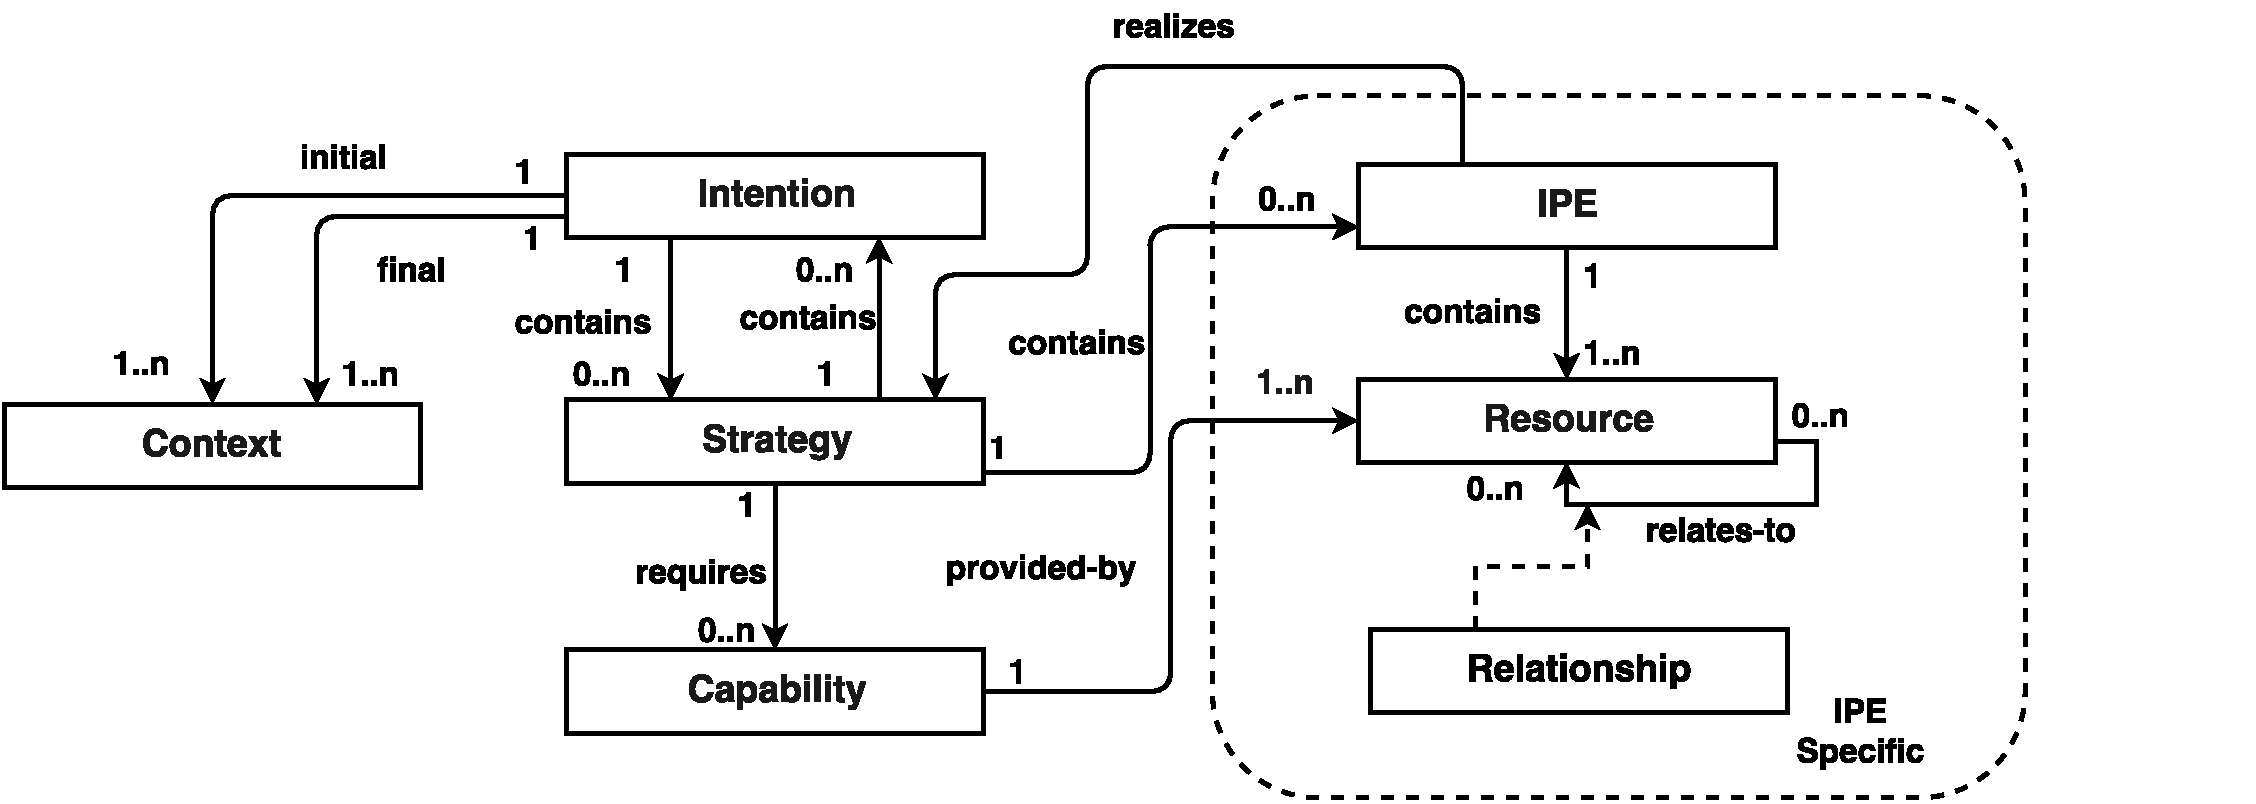
\includegraphics[width=1.1\textwidth]{entity.pdf}
	\caption{Organizational Modeling Entity Types Representation}
	\label{fig:entitymodel}
\end{figure}

In Sungur et al \cite{Sungur2014a} work, the concept of \textit{Informal Process Support Model} (IPSM) has been introduced which is to make use of existing knowledge of human performers. Here the initial creator of the model is experienced human performers. Based on their experience, they add relevant  resources of an informal process. The models are generated at runtime based on the interactions and activities of corresponding human performers. An informal process targets for accomplishment of an intention. The intentions can be refined by defining sub-intentions and/or strategies, which can then be further refined recursively as independent informal processes. The intention-based approach enables describing processes declaratively, i.e., without describing \textit{how} the intention is achieved, and providing only information about \textit{what} is achieved. As the author \cite{Sungur2014a} suggests that this avoids need of predefined business logic in the representations of informal processes. Each resource can be related to another resource in the context of an informal process using predefined or custom \textit{Relationships}. Informal Process Essentials are realized through strategies. Each informal process starts from an initial context, i.e., \textit{initial context} and aims to achieve an intention. After accomplishing the intention, there is a resulting context called as \textit{final context}. The beginning state before achieving intention is called as initial context and the end state after achieving intention is called as final context. On completion of intention execution, the process state changes from one state to another.

%%%%%%%%%%%%%%%%%%%%%%%%%%%%%%%%%%%%%%%%%%%%%%%%%%%%%%%%%%%%%%%%%%%%%%%%%
\section{Second Phase of InProcXec}
\label{sec:inproxec}
%%%%%%%%%%%%%%%%%%%%%%%%%%%%%%%%%%%%%%%%%%%%%%%%%%%%%%%%%%%%%%%%%%%%%%%%%
In this section, we present an overview about the \textit{Executing Informal Processes} (InProXec) method, proposed by Sungur et al. \cite{Sungur2015}. Since this thesis work is realizing resource-centric modeling of organizations, the main focus of this section is on the second phase of InProXec which is \textit{Informal Process Modeling}(P2). The method described in Figure \ref{fig:inprocxec_steps}, initializes informal process models in an automated fashion. The author also proves feasibility of the approach with a suitable case study.  In the following paragraphs, a short overview about different phases of the InProXec method has been provided and with a detailed description about the second phase of the \textit{InProXec} method. 

\begin{figure}
	\centering
	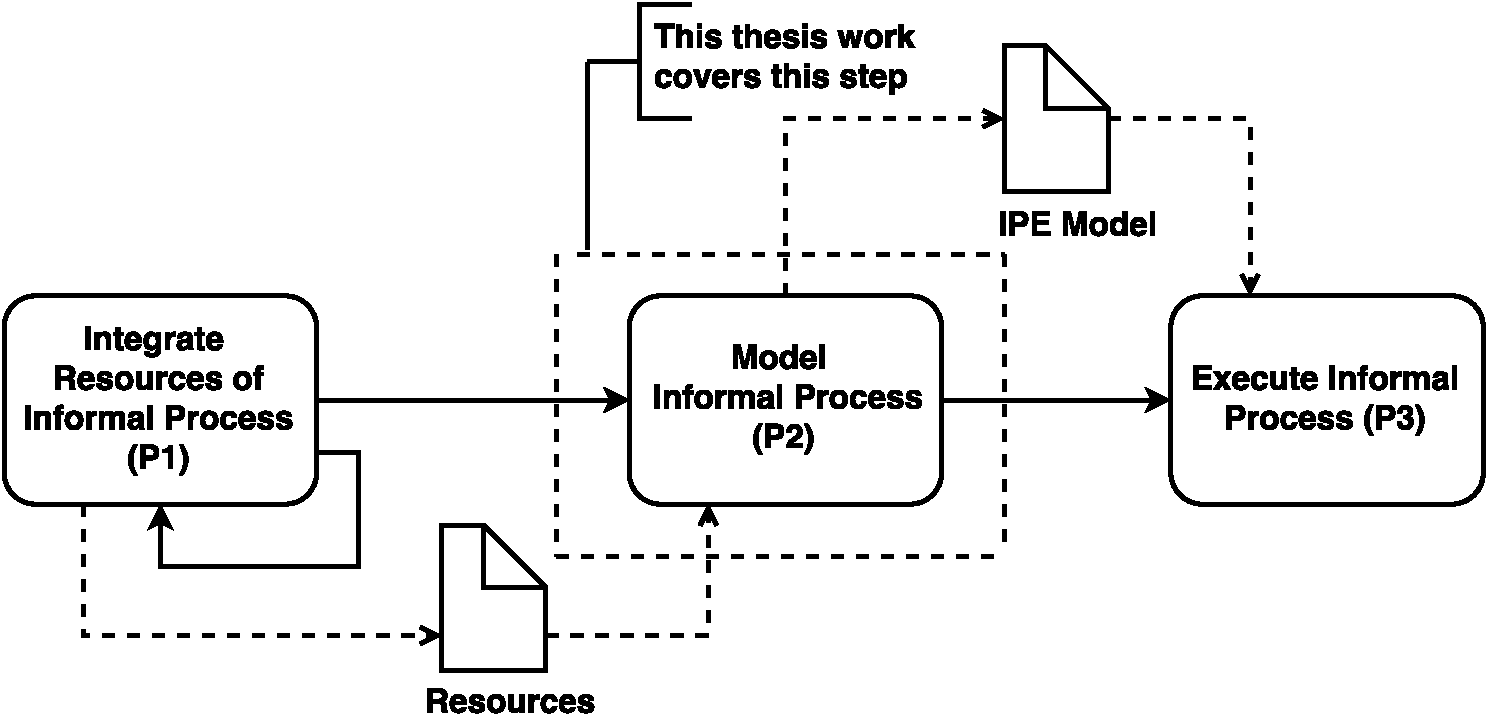
\includegraphics[width= \textwidth]{InProXec_Steps.pdf}
	\caption{Steps of the InProXec approach \cite{Sungur2015}}
	\label{fig:inprocxec_steps}
\end{figure} 

As shown in the Figure \ref{fig:inprocxec_steps}, the InProcXec method consists of four different phases:

\textit{Integrate Resources of Informal Processes (P1)} - In order to model an informal process, we need information about resources and its associated entities. The required information are collected beforehand during process execution. There exist many services to acquire information about informal processes resources automatically. The final output of this phase is \textit{integrated resources} which are required as an input to next modeling phase P2. Thus this phase sets up an environment required for modeling and execution of informal processes.  

\textit{Model Informal Processes (P2)} - This phase receives resource definitions made available in the first phase P1 as an input.  Based on this, business experts model informal processes and associated entities like strategies, intentions, capabilities etc., using our developed web editor. This phase has been explained in detail in the following sub section \ref{subsec:informalprocessmodeling}    

\textit{Execute Informal Processes (P3)} - The previous phase P2, describes only the intentions required to be achieved, corresponding required resources etc. In phase P2, the functionality to instantiate acquirable entities are not included. Thus in third phase P3, the output of phase P2 is taken i.e IPE models and are transformed into intializable self-contained \textit{Deployable Informal Process Essentials Archives(DIPEA)} \cite{Sungur2015} takes place. This results in DIPEAs enacting required informal process. To realize, phase P3 an \textit{IPE Model Compiler} also been introduced in the approach. 

\textit{Informal Process Model Deployment and Runtime (P4)} This phase employs \textit{IPE Runtime} which parses DIPEAs and runs the executables contained in those archives. During this phase, the autonomous actors work towards intentions of informal processes using acquired resources and other involved resources.  











